% !TeX program = pdflatex
% !TeX encoding = UTF-8
% !TeX spellcheck = es_ES

\documentclass[9pt, handout]{beamer}

%********************************************************************
% Packages
%********************************************************************

\usepackage[utf8]{inputenc}
\usepackage[T1]{fontenc}
\usepackage[english]{babel}
\usepackage[bottom, para]{footmisc}
\usepackage{amsmath,amssymb,amsthm}
\usepackage{graphicx}
\usepackage{hyperref}
\usepackage{listings}
\usepackage{perpage}
\usepackage{xcolor}
\usepackage{wrapfig}
\usepackage{ifthen}
\usepackage{scrextend} % add margin to answers
\usepackage{dashrule}

%********************************************************************
% Packages options
%********************************************************************

% geometry
\usepackage{geometry}
\geometry{
    a4paper,
    ignoremp,
    bindingoffset = 1cm, 
    textwidth     = 13.5cm,
    textheight    = 21.5cm,
    lmargin       = 1cm,
    rmargin		    = 3cm,
    tmargin       = 2cm,
    bmargin       = 3cm
}

% listings
\renewcommand{\lstlistingname}{Code}

\definecolor{lightgray}{rgb}{.9,.9,.9}
\definecolor{darkgray}{rgb}{.4,.4,.4}
\definecolor{purple}{rgb}{0.65, 0.12, 0.82}
\lstset{
  basicstyle=\small\sffamily,
  numbers=left,
  numberstyle=\tiny,
  numbersep=3pt,
  stepnumber=1,
  frame=tb,
  columns=fullflexible,
  backgroundcolor=\color{yellow!15},
  keywordstyle=\color{blue}\bfseries,
  ndkeywordstyle=\color{darkgray}\bfseries,
  identifierstyle=\color{black},
  commentstyle=\color{purple}\ttfamily,
  stringstyle=\color{red}\ttfamily,
  numberbychapter=false,
  showstringspaces=false,
  breaklines=true,
  captionpos=b, % put captions at the bottom 
}
%\lstset{
%  numbersep=5pt,
%  frame=trbl
%}

\definecolor{prismgreen}{rgb}{0.12, 0.48, 0.12}
\lstdefinelanguage{prism}{ % syntax highlight via font
  keywords={
    bool,C,ceil,const,ctmc,double,dtmc,endinit,endmodule,endrewards,endsystem,F,false,floor,formula,G,global,I,init,int,label,max,mdp,min,module,nondeterministic,P,Pmin,Pmax,prob,probabilistic,R,rate,rewards,Rmin,Rmax,S,stochastic,system,true,U,X
  }, 
  keywordstyle={\bfseries\color{black}}, 
  numberstyle=\tiny\color{black}, 
  comment=[l] {//}, morecomment=[s]{/*}{*/}, % single and multi-line 
  commentstyle= \color{prismgreen}, % dark green 
  tabsize=4, % tab treatment (going to be fixed in Prism)
  escapechar=@ % write LaTeX comments escaped by @ symbol 
} 

% perpage
\MakePerPage{footnote}

% hyperref
\definecolor{webgreen}{rgb}{0,.5,0}
\definecolor{webbrown}{rgb}{.6,0,0}
\definecolor{RoyalBlue}{cmyk}{1, 0.50, 0, 0}
\hypersetup{%
  %draft, % = no hyperlinking at all (useful in b/w printouts)
  colorlinks=true, linktocpage=true, pdfstartpage=3, pdfstartview=FitV,%
  % uncomment the following line if you want to have black links (e.g., for printing)
  % colorlinks=false, linktocpage=false, pdfstartpage=3, pdfstartview=FitV, pdfborder={0 0 0},%
  breaklinks=true, pdfpagemode=UseNone, pageanchor=true, pdfpagemode=UseOutlines,%
  plainpages=false, bookmarksnumbered, bookmarksopen=true, bookmarksopenlevel=1,%
  hypertexnames=true, pdfhighlight=/O,%nesting=true,%frenchlinks,%
  urlcolor=RoyalBlue, linkcolor=black, citecolor=webbrown, %pagecolor=RoyalBlue,%
  %urlcolor=Black, linkcolor=Black, citecolor=Black, %pagecolor=Black,%
}

% graphicx
\graphicspath{{img/}}

%********************************************************************
% New commands
%********************************************************************

\newcommand{\question}[1]{%
  \vspace{20pt}%
  \begin{wrapfigure}{l}{0.1\textwidth}%
    \vspace{-30pt}%
    \begin{center}%
      
\includegraphics[scale=1]{hand.jpg}%
    \end{center}%
    \vspace{-30pt}%
  \end{wrapfigure}%
  \noindent #1%
}%
\newcommand{\answer}[1]{%
  \vspace{5pt}\par\noindent
  \textbf{\underline{Answer:}}%
  \begin{addmargin}[1em]{1em}% 1em left, 2em right
    #1%
    \begin{flushright}%
      \qedsymbol%
    \end{flushright}%
  \end{addmargin}%
}%

\definecolor{light-gray}{gray}{0.95}
\newboolean{inlineCodeBackground}
\setboolean{inlineCodeBackground}{false}
\newcommand{\prism}[1]{%
  \ifthenelse{\boolean{inlineCodeBackground}}{%
    \colorbox{light-gray}{\lstinline[language=prism]{#1}}%
  }{%
    \lstinline[language=prism]{#1}%
  }%
}%
\newcommand{\bash}[1]{%
  \ifthenelse{\boolean{inlineCodeBackground}}{%
    \colorbox{light-gray}{\lstinline[language=bash]{#1}}%
  }{%
    \lstinline[language=bash]{#1}%
  }%
}%

\newcommand{\dashedrule}{%
  \noindent\hdashrule{\textwidth}{1pt}{1.5mm}%
}%


\title[AAL basada en modelos]{Ambient Assisted Living basada en modelos}
\author{\textbf{Tommaso Papini}}
\institute{
  STLab, Departamiento de la Ingenieria de la Informacíon, Universidad de Florencia, Italia,\\
  {tommaso.papini@unifi.it}
}
\date{
  29 de Mayo 2017\\
  {\small Departamento de Informática, Universidad de Jaén, España}
}

\begin{document}

  \begin{frame}
    \titlepage
    \begin{itemize}
      \item Análisis cuantitativa basada en modelos
      \item Reconocimiento de Actividades
%      \begin{itemize}
%        \item diagnosis
%        \item predicción
%        \item planificación de acciones
%      \end{itemize}
%      \item Datasets para AAL
    \end{itemize}
  \end{frame}

  \begin{frame}{Overview}
    %\tiny
    \tableofcontents
  \end{frame}
  
  \section{Análisis cuantitativa basada en modelos}
    
    \subsection{Redes de Petri}
      \begin{frame}{TODO!!!}
      \end{frame}
      
    \subsection{Análisis de transición}
      \begin{frame}{TODO!!!}
      \end{frame}

  \section{Reconocimiento de Actividades}
  
    \begin{frame}{Dos artículos principales}
      \pause
      \begin{itemize}
        \item Carnevali, L., Nugent, C., Patara, F. and Vicario, E., 2015, September. \textbf{A continuous-time model-based approach to activity recognition for ambient assisted living}. In International Conference on Quantitative Evaluation of Systems (pp. 38-53). Springer International Publishing.
        \pause
        \item Biagi, M., Carnevali, L., Paolieri, M., Patara, F. and Vicario, E., 2016, October. \textbf{A Stochastic Model-Based Approach to Online Event Prediction and Response Scheduling}. In European Workshop on Performance Engineering (pp. 32-47). Springer International Publishing.
      \end{itemize}
    \end{frame}
    
    \begin{frame}{Reconocimiento de Actividades}
      \pause
      Un \textit{entorno inteligente} (es decir, dotado de sensores y actuadores) es un sistema \textbf{parcialmente observable}:
      \pause
      \begin{itemize}
        \item el estado efectivo del sistema resulta escondido
        \pause
        \item solo se pueden observar eventos (\textit{observaciones}) emitidos por el sistema (por ej. la activación de un sensor)\\[1em]
      \end{itemize}
      
      \pause
      
      Reconocimiento de Actividades:
      \pause
      \begin{itemize}
        \item \textbf{Diagnosis}: estimar cual es el estado efectivo actual del sistema a partir de las observaciones registradas
        \pause
        \item \textbf{Predicción}: estimar cual será el estado efectivo del sistema después de una determinada cantidad de tiempo
        \item \textbf{Planificación de acciones}: elegir la acción optima y entre cuanto tiempo ir actuarla para evitar situaciones críticas\\[1em]
      \end{itemize}
    \end{frame}
    
    \begin{frame}{Reconocimiento de Actividades}
      \begin{center}
        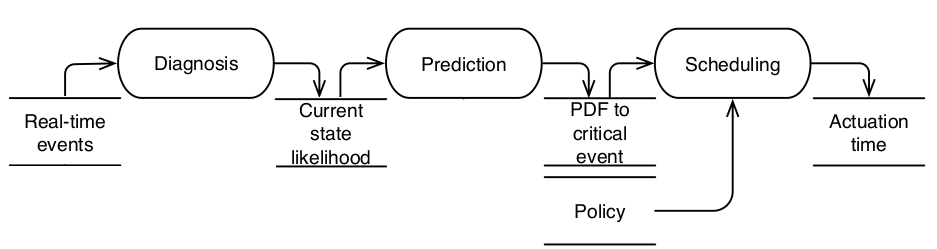
\includegraphics[scale=0.35]{img/diag_pred_sched_chain_general.png}
      \end{center}
      
      \pause
            
      El Reconocimiento de Actividades es fundamental en el desarrollo de sistemas inteligentes en cuanto actúa de puente entre los datos recibidos por los sensores y la semántica de alto nivel de las aplicaciones.
    \end{frame}
    
    \subsection{Diagnosis y predicción}
      
%      \begin{frame}{HMM y CRF}
%        \pause
%        Los \textit{Modelos Ocultos de Márkov} (HMM, Hidden Markov Model) y los \textit{Campos Aleatorios Condicionales} (CRF, Conditional Random Field) ofrecen soluciones clásicas para realizar diagnosis y predicción en sistemas parcialmente observables en tiempo \textbf{discreto}.\\[1.5em]
%        
%        \pause
%        
%        El objetivo principal de las técnicas basadas en modelos para sistemas parcialmente observables es realizar la misma diagnosis y predicción, pero en tiempo \textbf{continuo}.
%      \end{frame}
      
      \begin{frame}{Diagnosis y predicción con modelos}
        \pause
        La idea es explotar las técnicas de análisis cuantitativa basada en modelos para realizar diagnosis y predicción.\\[1em]
        
        \pause
        
        Pasos principales:
        \pause
        \begin{enumerate}
          \item Obtener a un dataset de observaciones \textit{anotado} (es decir, con observaciones y actividades efectivas en un intervalo de tiempo)\footnote{Van Kasteren, T., Noulas, A., Englebienne, G. and Kröse, B., 2008, September. \textbf{Accurate activity recognition in a home setting}. In Proceedings of the 10th international conference on Ubiquitous computing (pp. 1-9). ACM.}
          \pause
          \item Calcular medidas estadísticas
          \begin{itemize}
            \item correlación entre eventos y actividades
            \item duración de actividades
            \item inter-tiempo entre eventos durante actividades
          \end{itemize}
          \pause
          \item Construir a un modelo del sistema
          \begin{itemize}
            \item process elicitation
            \item process enhancement
          \end{itemize}
          \pause
          \item Análisis de transición
        \end{enumerate}
      \end{frame}
        
    \subsection{Planificación de acciones}
      \begin{frame}{TODO!!!}
      \end{frame}
            
%  \section{Datasets para AAL}
%    
%    \subsection{TODO!!!}
%      \begin{frame}{TODO!!!}
%      \end{frame}

\end{document}
